\documentclass[a4paper,12pt]{article}

% % Document setup
\usepackage[a4paper]{geometry}
\setlength{\parskip}{1.5ex plus 0.5ex minus 0.5ex}

% % Language and typography
\usepackage{tipa}
\usepackage{amsmath}

% % Graphics and colors
\usepackage{graphicx}
\usepackage[table,xcdraw]{xcolor}

% % Bibliography and referencing
\usepackage[style=apa,sorting=nyt]{biblatex}
\usepackage{footnotebackref}

% Miscellaneous
\usepackage{tfrupee} % For rupee symbol
\usepackage{multirow} % For tables
\usepackage{fancyhdr} % For custom headers
\usepackage{titling}
\usepackage{hyperref}
\addbibresource{references.bib}
\hypersetup{
    colorlinks=true,      % Enable colored links
    linkcolor=blue,   % Color of internal links
    citecolor=blue,   % Color of citations
    urlcolor=blue,    % Color of URLs
}

% % Remove page number on cover page

\title{\LARGE The Himalayan Tightrope:\\ \Large Balancing Growth and Sustainability amidst\\ Ecological Sensitivity}
\author{Ritwiz Sarma\thanks{Corresponding author. Email: ge23ritwiz@mse.ac.in. This is a preliminary draft for the 59th Conference of the Indian Econometric Society. Do not cite.}\\\small~Madras School of Economics \and Riju Garg\thanks{Email: ge23riju@mse.ac.in.}\\\small~Madras School of Economics} % Riju can add acknowledgements and contact details here.
% \predate{Latest version available \href{www.facebook.com}{here}\\[1cm]}
\date{This version: January 14, 2025}


\begin{document}
\pagestyle{empty}
\maketitle
\begin{abstract}

    Is there a trade-off between economic growth and environmental preservation? This study uses high-resolution (town/village-level) satellite data to analyse the new relationships emerging between environmental sustainability and growth in the specific context of infrastructure development, for which we build a novel dataset for five economic and environmental indicators over two decades. Our focus is on the ecologically-sensitive Himalayan biome, and specifically on the states of Himachal Pradesh and Uttarakhand, which have experienced significant infrastructure growth over the study period. We capture highly-localized effects and find significant heterogeneities across time, which have implications for sustainable development and decentralized policymaking.

\end{abstract}
\vfill
\textit{Keywords}: Infrastructure, Growth, Sustainable Development, Remote Sensing, Economy-Ecology Tradeoff
% \begin{center}
%     \footnotesize Something.
% \end{center}
\newpage
\newgeometry{margin=1in}
\pagestyle{plain}

\section{Introduction}

% to be rewritten and lengthened

Over the past few decades, the growth of environmental awareness has often conflicted with voices urging for development, courtesy of often contrasting perspectives on the relation between environmental sustainability and economic growth \parencite{arrow1995,grossman1991,grossman1995,list1999,selden1994,shafik1992}. The investigation of this relationship has often used the environmental Kuznets curve, which hypothesizes an inverted-U shaped relationship between growth and environmental degradation. This paper uses new-age satellite-based data sources to reconstruct and analyse the environmental Kuznets formulation for a specific biome of exceeding importance, the Himalayas.

The Himalayan mountain range – often called the “third pole” - has always been considered a boon to India in terms of the natural resources, economic support, and natural defence that it provides \parencite{dyola2024}. Development in the Himalayas, however, has been controversial: on one hand, there has been rapid infrastructural development and investment by the government, in order to increase the connectivity of the Himalayan states with the rest of the country and extract more economic benefits through avenues such as tourism (ibid.). On the other hand, nudges to the fragile environmental ecosystem of the Himalayas have been connected to their increased vulnerability to disasters - the most notable example being the 2023 land subsidence incident at Joshimath, Uttarakhand \parencite{sharma2023}.

This study uses high-resolution geospatial data, which allows us to narrow our focus to the Himalayan states of Himachal Pradesh and Uttarakhand, while preserving richness in the data to make statistical inference possible. Our novel construction of the EKC is at the village/census town level, compared to previous estimations made from large-scale macroeconomic data at the level of countries or states (for example, \cite{caviglia2009,kalka2013,list1999}). This allows us to account for localized heterogeneities, which are particularly important in this ecologically sensitive region. We trace the paths of development and ecological degradation and find contrasting relationships across different periods, even as growth processes grow seemingly unabated.

The following section provides further context on the economy-environment trade-off and its intersection with the Indian policy backdrop. The third section describes our data across our temporal range and introduces our panel model to study the impacts of change in the environmental indicators on the night-time lights data, which is being used as a signal of infrastructure development. The fourth section summarizes our results, and the final section concludes.


\section{Context: Why Build Infrastructure?}

The infrastructural development of the Himalayan region is vital for India from three perspectives: economic, political, and administrative. We provide general outlines for the latter two and focus primarily on the first.

The Himalayas are located on India’s border with China, Nepal, and Bhutan. This has spurred numerous infrastructural programmes, including the India-China Border Roads (ICBR) built since 1997 \parencite{mha_n.d.} in response to Chinese infrastructure development along the border. The project includes construction of strategic roads, including bridges and tunnels, for commuting of artillery and infantry, thereby ensuring increased security. Thus, from the administrative perspective, building infrastructure becomes essential to strengthen the reach of the state. For example, during a natural calamity, relief efforts become more convenient to carry out in the presence of better infrastructure.

From a political perspective, road building in particular remains a favoured form of public investment, mainly because of its visible nature which promises electoral returns \parencite{berg2015}. Moreover, local economic conditions may call for politically motivated investment. In Uttarakhand, a shift is taking place from being an agriculture-based economy to one focusing on manufacturing and services. The primary sector provided for 10.2\% of GSDP in 2019-20 – a steep fall from a lofty 31.49\% in 1999-2000 \parencite{directorate2021}. As for Himachal Pradesh, provision of livelihoods has increasingly become a political concern, especially since no political party has dominated state elections \parencite{kumar2022}. Thus, by investing in infrastructure development, policymakers may claim a stimulus effect for the local economy hoping to attract voters.

The economic motivation views infrastructure investment in the Himalayan region as key to development. The United Nations Environment Programme divides mountain infrastructure into three categories: Access, Communication, and Energy to highlight their importance as agents of change \parencite{kohler2002}. The following can be considered as the main examples of the three categories respectively: roads, telecom services \& internet, and dams. Roads are essential amidst the mountainous terrain to improve connectivity and provide livelihoods through tourism. Telecom services and internet connectivity improve the communication of the states and bridge the digital gap, promoting better education and health care facilities as well. Hydroelectric power plants provide energy that is essential for local development. We expand more on our view of infrastructure and growth in the following section.

It remains true that the Himalayan states have a record of natural calamities propelled by development processes: the 2013 Uttarakhand floods prompted discussion on overexploitation of natural resources and the awareness for sustainable development. Ten years later, the Himalayan region was struck by the Joshimath land subsidence incident in 2023. Though the government has tried to initiate programmes like Himalaya Diwas \parencite{press2021} to protect the ecosystem, the results have not been satisfactory.


\section{Theoretical Framework}

The environmental Kuznets curve (EKC) was introduced with the hypothesis that there exists an inverted-U relationship between environmental degradation and national income. It was developed by \textcite{grossman1991} who analyzed the linkage between economic growth and environmental pollution. Using indicators on air pollution and contamination of river basins, they postulated that the initial stages of economic growth are associated with increased environmental degradation due to increased exploitation of natural resources, production, and industrialization and thus environmental degradation may be inevitable in developing regions where countries have either embarked on or are in the process of embarking on the path to development.

\begin{figure}[h]
    \centering
    \includegraphics[width=0.7\textwidth]{images/kuznets_scen.png}
    \caption{Different scenarios for the Environmental Kuznets curve (Dasgupta et al., 2002).}
    \label{fig:kuznets}
\end{figure}

However, there is a significant body of work contradicting the inverted-U hypothesis. \textcite{stern2004} points out that the EKC is econometrically weak and that the empirical support for the EKC is mixed. \textcite{dasgupta2002} presented evidence that contradicted the typical EKC pattern (Figure \ref{fig:kuznets}). Similarly, the shape of the Kuznets curve has been disputed over the past decades \parencite{caviglia2009,kalka2013,list1999}. In short, while the inverted-U essentially predicts that economies will “grow out of” \parencite{shafik1992} environmental damage, this does not necessarily follow. Achieving growth is therefore not a panacea for environmental loss, no matter how appealing the counterfactual may be.

The existing literature has mostly used indicators like air quality, emissions, and particulate matter to study environmental degradation as a proxy to analyze economic growth. \textcite{caviglia2009} use Ecological Footprint (EF) as a measure of environmental degradation. However, in this paper, we also include forest cover as an indicator for environmental degradation. Forest cover is a respected measure of environmental sustainability \parencite{wang2003}. For example, the Finance Commission of India, which rewards efforts made towards environmental sustainability for horizontal devolution of funds, uses forest cover as the sole metric \parencite{finance2020}.

Our focus throughout this study is the role of infrastructure growth, for which we present several motivations. Infrastructure growth, in the form of transportation systems and urbanization, is generally hypothesized as a catalyst for environmental degradation in the Himalayas \parencite{prashar2023,singh2005}. Moreover, the long-run effects of environmental degradation are inescapably infrastructure decay - landslides regularly block roads \parencite{mey2023} and render public funds spent on connectivity worthless. Nonetheless, public infrastructure investment as a pathway to growth is an accepted ‘stylized fact’ and has been empirically demonstrated as true for the Himalayan region in particular (e.g., \cite{tiwari2000}). Political and administrative incentives also align with infrastructure investment, as mentioned in Section 2.1. We therefore use night-lights and built-up area using publicly available satellite data to measure what we term as “infrastructure-led economic growth” (ILEG). ILEG reflects ground-level infrastructure development at a high resolution and provides a suitable measure of overall growth. We expand on our data further in the next section.


\section{Data}


% Table created by stargazer v.5.2.3 by Marek Hlavac, Social Policy Institute. E-mail: marek.hlavac at gmail.com
% Date and time: Fri, Jan 17, 2025 - 02:12:05
\begin{table}[b] \centering 
  \caption{Descriptive statistics.} 
  \label{tab:desc} 
\begin{tabular}{@{\extracolsep{5pt}}lrrrr} 
\\[-1.8ex]\hline 
\hline \\[-1.8ex] 
Statistic & \multicolumn{1}{c}{Mean} & \multicolumn{1}{c}{St. Dev.} & \multicolumn{1}{c}{Min} & \multicolumn{1}{c}{Max} \\ 
\hline \\[-1.8ex] 
% year & 652,620 & 2,010.500 & 5.766 & 2,001 & 2,020 \\ 
Night lights   &  6.471 & 6.525 & 0.000 & 63.000 \\ 
PM2.5 pollution &  30.542 & 6.748 & 12.386 & 77.000 \\ 
Forest cover   &  75.112 & 10.964 & 20.381 & 100.000 \\ 
Land surface temperature   &  292.511 & 3.050 & 264.125 & 300.335 \\ 
Built-up area  &  118.525 & 204.381 & 0.000 & 3,917.117 \\ 
\hline \\[-1.8ex] 
\end{tabular} 
\end{table} 


% \begin{table}[b]
%     \centering
%     \begin{tabular}{|l|r|r|r|r|}
%     \hline
%     \multicolumn{1}{|c|}{\textbf{Variable}} & \multicolumn{1}{c|}{\textbf{Mean}} & \multicolumn{1}{c|}{\textbf{Std. Dev.}} & \textbf{Min} & \textbf{Max} \\ \hline
%     Built-up area                           & 69.70                             & 107.06                                  & 0.00            & 1570.46      \\ \hline
%     Night-lights                            & 2.19                              & 4.21                                   & 0.00            & 63.00           \\ \hline
%     Forest cover                            & 24.89                              & 8.42                                    & 79.62        & 120.00          \\ \hline
%     PM2.5                                   & 31.50                              & 7.83                                    & 12.79        & 77.00           \\ \hline
%     LST                                     & 25.51                             & 9.23                                   & 21.42       & 36.20       \\ \hline
%     \end{tabular}
%     \caption{Descriptive statistics.}
% \end{table}

Our smallest unit of measurement is the shrid, an area unit used by the Socioeconomic High-resolution Rural-Urban Geographic Platform for India (SHRUG). It is a village or town unit that has had consistent borders since 1991. This subnational resolution allows us to vastly expand the statistical power of our tests, which becomes relevant in our estimation tasks later.

For studying economic growth, we use night-time lights and built-up area (Table 1). Night-time lights data has been used to generate measures of economic activity from the early 1990s. Satellite night-time light data offers a unique and comprehensive view of the entire planet, enabling the identification of energy access and quality gaps, as well as trends in economic activity. The remote sensing and economics literature suggests a strong correlation between night-time lights and GDP growth, even at the subnational level, as \textcite{doll2006} find for the regional GDP of 11 European Union countries and US GDP at the state level. We use two sources for night-lights: the Defense Meteorological Program Operational Line-Scan System (DMSP-OLS) and the Visible Infrared Imaging Radiometer Suite (VIIRS) instrument. DMSP-OLS has the unique capability to detect visible and near-infrared emission sources at night, while VIIRS data is a new consistently processed time series of annual global night-time lights that has been produced from monthly cloud-free average radiance grids.
Built-up area is also obtained from high-resolution daytime satellite data. It leverages a particular type of land use associated with urbanization. It is also used for detecting economic activity at highly local levels - which is particularly useful for developing countries where infrastructure growth is especially likely to spur economic growth. \textcite{baragwanath2021} is an example of a similar use case. We obtain our built-up area estimates from the GHSL (Global Human Settlement) framework provided by the Copernicus Data Space Ecosystem.
For environmental degradation, we measure air quality, forest cover, and land surface temperature (LST). Surface PM 2.5 is the estimated annual ground level fine particulate matter by combining Aerosol Optical Depth (AOD) retrievals from the NASA MODIS, MISR and SeaWIFS instruments with the GEOS-Chem chemical transport model. The satellite-based Vegetation Continuous Fields (VCF) is used for measuring global forest cover change. It is usually a key parameter for a variety of environmental and climate related applications. LST serves as a predictor for global warming.


\section{Findings}

\subsection{Temporal Shifts}

\subsubsection*{Himachal Pradesh}

\begin{description}
    \item[Forest Cover] From the early 2000s to the mid-2000s, there was a noticeable increase in forest cover in the northern districts of Kullu, Chamba, and Kinnaur. In contrast, urbanization continued to progress in the southern districts, including Una, Hamirpur, Solan, and Bilaspur, leading to a reduction in forest cover in these areas. Notably, Shimla experienced a decline in forest cover during this period. In other regions, the forest cover remained relatively stable. By the 2010s, however, a positive trend in forest cover emerged in the southern regions as well. The period from 2010 to 2015 marked a significant shift, with most districts witnessing changes in forest cover.
    \item[Nighttime lights] There is a discernible trend of increasing nighttime lights across the periods from the early 2000s to the mid-2000s, and from 2010 to the mid-2010s, which indicates a pattern of higher economic growth during these times.

\end{description}

\begin{figure}[h]
    \centering
    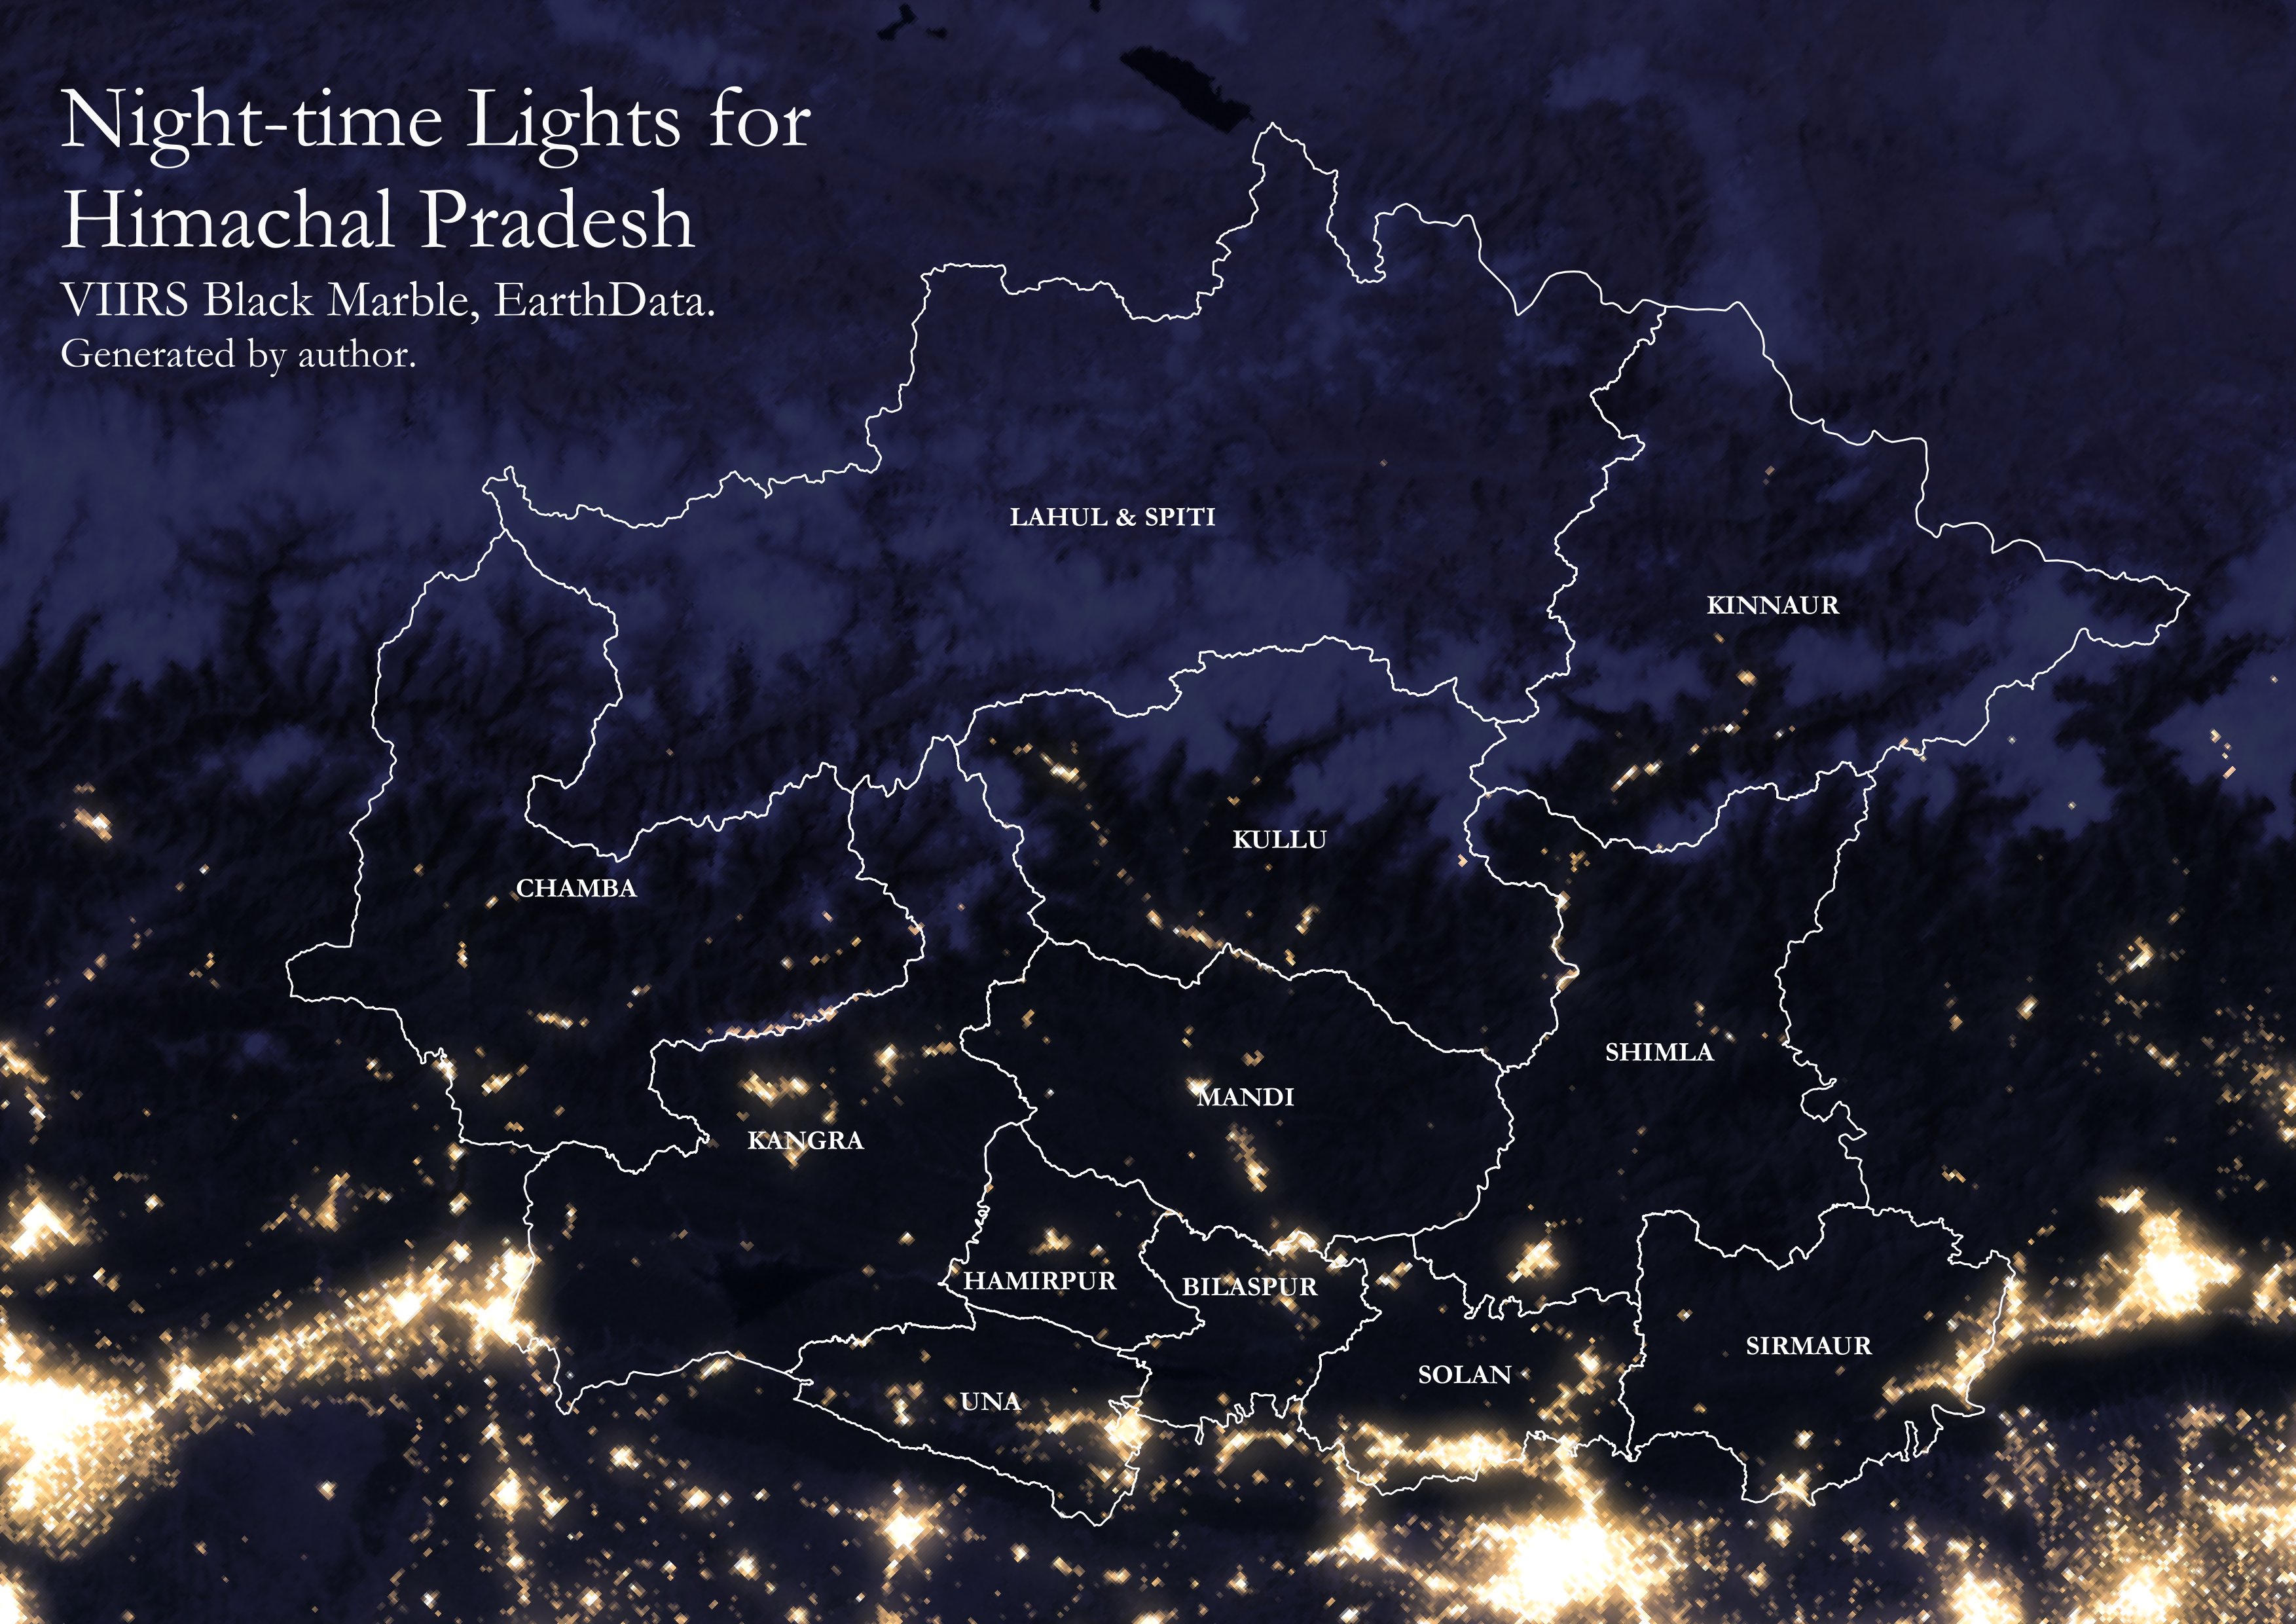
\includegraphics[width=0.85\textwidth]{images/ntl_hp.png}
    \caption{Nighttime lights for Himachal Pradesh.}
\end{figure}


\subsubsection*{Uttarakhand}

\begin{description}
    \item[Forest Cover] The state exhibits a heterogeneous pattern of forest cover growth. From the early 2000s to the mid-2000s, the trend mirrored that of Himachal Pradesh, with increasing forest cover in the northern districts and a decline in the southern districts, notably Haridwar and Rudrapur. However, from the mid-2000s to the 2010s, the forest cover decreased across the state. After 2010, a resurgence in forest cover growth was observed.
    \item[Nighttime lights] Night lights increased gradually from the early 2000s to the mid-2000s. However, from the mid-2000s to the early 2010s, there was a more pronounced growth in night-time light intensity, depicting higher economic growth.

\end{description}

\subsection{Results}

We estimate a simple model of the EKC, using our compound indices across 32,634 \textit{shrids} located within the two states. First, we construct our indices with equal weights $w_i$ across variables:

\begin{align*}
    \rm{EconIndex}_i &=  w_1(\rm{NTL}_i) + w_2(\rm{Builtup}_i) \\
    \rm{EnvIndex}_i &=  w_1(\rm{AQI}_i) + w_2(\rm{ForestCover}_i) + w_3(\rm{LST}_i)
\end{align*}

where $\sum_{i=1}^{n}w_i = 1$ and $w_i = w_j \forall i, j$ for each Index. We run the Hausman test and find that the fixed effect estimators are more suitable for our data. Thus, we estimate a quadratic fixed-effects model in two epochs:

\[
    \rm{EconIndex}_{it} = \beta_0 + \beta_1(\rm{EnvIndex}_{it}) + \beta_2(\rm{EnvIndex}_{it}^2) + \eta_i + \epsilon_{it} 
\]

where $\eta_i$ represents individual (\textit{shrid}-specific) fixed effects and $\epsilon_{it}$ represents the stochastic error term.

\begin{table}[h]
    \centering
    \begin{tabular}{l|rrrr}
    \hline
    \multicolumn{1}{c}{\textbf{}} & \multicolumn{1}{c}{\textbf{Coef.}} & \multicolumn{1}{c}{\textbf{Std. Err.}} & \multicolumn{1}{c}{\textbf{t}} & \textbf{P\textgreater{}t} \\ \hline
    EconIndex                     & 0.0242\textsuperscript{***}                             & 0.0004                                 & 61.547     & 0.000                     \\ 
    EconIndex$^2$                   & -0.0002\textsuperscript{***}                            & 0.0001                                 & -18.148    & 0.000                    
    \\ \hline        
\end{tabular}
\caption{First epoch regression results. *** represent significance at the 1\% level.}
\label{tab:epoch1}
\end{table}

\begin{table}[h]
    \centering
    \begin{tabular}{l|rrrr}
    \hline
    \multicolumn{1}{c}{\textbf{}} & \multicolumn{1}{c}{\textbf{Coef.}} & \multicolumn{1}{c}{\textbf{Std. Err.}} & \multicolumn{1}{c}{\textbf{t}} & \textbf{P\textgreater{}t} \\ \hline
    EconIndex                     & -0.2366\textsuperscript{***}                             & 0.0332                                 & -7.1136     & 0.000                     \\ 
    EconIndex$^2$                   & 0.0073\textsuperscript{***}                            & 0.0016                                 & 4.7800    & 0.000                    
    \\ \hline        
\end{tabular}
\caption{Second epoch regression results. *** represent significance at the 1\% level.}
\label{tab:epoch2}
\end{table}

% 
% Table created by stargazer v.5.2.3 by Marek Hlavac, Social Policy Institute. E-mail: marek.hlavac at gmail.com
% Date and time: Sun, Jan 05, 2025 - 23:55:09
\begin{table}[hbt] \centering 
  \caption{Regression results from Model 1 for Epoch 1.} 
  \label{} 
\begin{tabular}{@{\extracolsep{5pt}}lccc} 
\\[-1.8ex]\hline 
\hline \\[-1.8ex] 
 & \multicolumn{3}{c}{\textit{Dependent variable:}} \\ 
\cline{2-4} 
\\[-1.8ex] & ntl\_mean\_st & ntl\_mean & ntl\_mean\_st \\ 
\\[-1.8ex] & (1) & (2) & (3)\\ 
\hline \\[-1.8ex] 
 env\_index & 0.144$^{***}$ &  &  \\ 
  & (0.00001) &  &  \\ 
  & & & \\ 
 env\_index\_sq & 0.068$^{***}$ &  &  \\ 
  & (0.00000) &  &  \\ 
  & & & \\ 
 VCF\_LST\_PC &  & 0.434$^{***}$ &  \\ 
  &  & (0.0004) &  \\ 
  & & & \\ 
 VCF\_LST\_PC$^2$ &  & 0.567$^{***}$ &  \\ 
  &  & (0.0001) &  \\ 
  & & & \\ 
 VCF\_LST\_UW &  &  & 0.097$^{***}$ \\ 
  &  &  & (0.00002) \\ 
  & & & \\ 
 VCF\_LST\_UW$^2$ &  &  & 0.179$^{***}$ \\ 
  &  &  & (0.00000) \\ 
  & & & \\ 
\hline \\[-1.8ex] 
Observations & 97,758 & 97,875 & 97,875 \\ 
R$^{2}$ & 0.120 & 0.101 & 0.101 \\ 
\hline 
\hline \\[-1.8ex] 
\textit{Note:}  & \multicolumn{3}{r}{$^{*}$p$<$0.1; $^{**}$p$<$0.05; $^{***}$p$<$0.01} \\ 
\end{tabular} 
\end{table} 


The regression results showcase a mixed response with respect to the Environmental Kuznets curve hypothesis. During the initial epoch (Table \ref{tab:epoch1}), the results are consistent with the EKC and the scatterplot is an inverse-U curve (Figure \ref{fig:epoch1}), that is economic growth and environment degradation, are both increasing until a certain level before the environment degradation starts to reduce.

With time, there is a deviation from this hypothesis. During the second epoch (Table \ref{tab:epoch2}), the results contradicted the EKC, with a U-shaped curve (Figure \ref{fig:epoch2}) indicating that as economic growth increases there is a fall in environmental degradation till a certain level. After that certain level is attained, the environmental degradation starts to rise again with economic growth.


\begin{figure}[h]
    \centering
    \includegraphics[width=0.7\textwidth]{images/kuznets.png}
    \caption{Estimated relationship for first epoch, similar to the EKC from Figure 1.}
    \label{fig:epoch1}
\end{figure}

\begin{figure}[h]
    \centering
    \includegraphics[width=0.7\textwidth]{images/notkuznets.png}
    \caption{Estimated relationship for second epoch, inverse of Figure 3.}
    \label{fig:epoch2}
\end{figure}


\section{Conclusion}

Our estimations result in an inverted U-shaped curve for the first epoch and a U-shaped curve for the second epoch. These inconsistent results imply presence of heterogeneity across time. While the initial period seems to conform to the traditional EKC hypothesis (inverted-U), the second period shows the opposite, with both results remaining statistically significant. Our evidence thus suggests that the economy-environment trade-off in the Himalayas is certainly more complex than the EKC suggests. 

Our primary takeaway from this result is that simplistic hypotheses are unlikely to be robust in ecologically sensitive areas, such as the Himalayas. The literature on development, as well as the lived experiences of several developing economies tell us that it is natural to face high environmental degradation during high economic growth. It is possible that ecological sensitivity is likely to increase the repercussions of developmental processes substantially, to the point where the compounded positive effects of growth no longer compensate for the ecological loss. 

An alternative, more worrying hypothesis is based on the fact that infrastructure growth (and by extension, ILEG) has consistently increased across our sample period. It is possible that the ecological dynamics of the area of interest may have reached a particular ‘tipping point’ - that is, the local relationship between economic growth and environmental degradation may have drastically changed over the past decade. A study focused on this phenomenon may unearth valuable results.

Like many other studies over the years focusing on the EKC, we benefit from recent advances in econometrics and data science to provide this novel analysis. The formulation of the EKC in literature has generally remained stable, which we have borrowed from as well. Our study gains from numerous statistical advantages - a balanced panel and large sample size, to name some - and thus illustrates data limitations (rather than theoretical loopholes) faced by previous studies.

To conclude, we reproduce List \& Gallet’s \parencite*{list1999} opinions on the policy importance of their study: “sustainable development strategies critically depend on well-informed policymakers.” Our work adds a vital new angle to this larger push towards evidence-based policymaking, viz., that local effects may diverge significantly from the overall. This adds a new imperative for third-tier policymakers. If the economy is facing a U-shaped curve, policymakers must focus on strategies to sustain growth while simultaneously reducing environmental degradation. Simple measures include switching to renewable sources of energy, solar plants, windmills which might be financially costly for developing countries but as a country attains growth, they can invest for environment protection \parencite{unep2023}. Other measures include encouragement of public transport as well as a switch to electric vehicles (ibid.).


\printbibliography

\end{document}
